% !TEX program = xelatex
\documentclass[UTF8, 10pt]{ctexrep}
% 中文排版设置
\ctexset{space=true, punct=quanjiao}

% 编程
\usepackage{ifthen}

% 颜色
\usepackage[dvipsnames]{xcolor}

% 字体
\usepackage{fontspec}
% \setmainfont[BoldFont={SourceHanSansSC-Medium}]{Source Han Serif SC}
\setCJKmainfont{Source Han Serif SC}
% \setsansfont[BoldFont={SourceHanSansSC-Bold}]{Source Han Sans SC}
\setCJKsansfont{Source Han Sans SC}
% \setCJKmonofont[BoldFont={Kaiti SC Bold}]{Kaiti SC Regular}

% 页面设置
\usepackage[papersize={13cm,18.4cm},hmargin=1.91cm,vmargin=2.24cm]{geometry}

% 页眉和页脚
\usepackage{fancyhdr}
\renewcommand{\chaptermark}[1]{\markboth{#1}{}}
\renewcommand{\sectionmark}[1]{\markright{\thesection\ #1}}
\fancyhf{}
\fancyfoot[C]{\thepage}
\fancyhead[LO]{\rightmark}
\fancyhead[RE]{\leftmark}
\renewcommand{\headrulewidth}{0pt} % 注意不用 \setlength
\renewcommand{\footrulewidth}{0pt}

% 章节样式
\usepackage{titlesec}
\titleformat{\chapter}
[hang]
{\sffamily\centering}
{\zihao{4} 第{\thechapter}章\enspace}
{0pt}
{\zihao{4} \bfseries}
[\vbox{\color{Melon}\titlerule \vspace{1pt} \titlerule}]
\titlespacing{\chapter}{0pt}{*0.2}{*0.3}

\titleformat{\section}[block]{\zihao{-4}\bfseries}{\S\thechapter.\arabic{section}}{1em}{}[]
% \titleformat{\subsection}[block]{\Large\itshape\mdseries}{\arabic{section}.\arabic{subsection}}{1em}{}[]
% \titleformat{\subsubsection}[block]{\normalsize\bfseries}{\arabic{subsection}-\alph{subsubsection}}{1em}{}[]
% \titleformat{\paragraph}[block]{\small\bfseries}{[\arabic{paragraph}]}{1em}{}[]

% 超链接
\usepackage{hyperref}
\hypersetup{
    colorlinks=true,
% linkcolor [red]
% anchorcolor [black]
% citecolor [green]
% filecolor [cyan]
% menucolor [red]
% runcolor [cyan - same as file color]
% urlcolor [magenta]
% allcolors -- use this if you want to set all links to the same color
}
% 交叉引用
\usepackage{nameref}
\usepackage{prettyref}
\newrefformat{fig}{图\ref{#1}}
\newrefformat{tab}{表\ref{#1}}
\newrefformat{cha}{第\ref{#1}章 \nameref{#1}}
\newrefformat{app}{附录\ref{#1} \nameref{#1}}

% 索引
\usepackage{makeidx}
\makeindex

% 图片
\usepackage{graphicx}

% 表格
\usepackage{array}
\usepackage{tabularx}
\usepackage{multirow}
\newcommand{\minitab}[2][l]{\begin{tabular}{#1}#2\end{tabular}}

% 列表
\usepackage{enumitem}
% \setlist{partopsep=2pt, itemsep=1pt, parsep=0pt}
% \setlist[itemize, 1]{align=left, labelindent*=1em, topsep={1pt plus 1pt minus 1pt}, itemsep={3pt plus 1pt minus 2pt}}
% \setlist[itemize, 2]{leftmargin=0em, topsep={2pt plus 2pt minus 1.5pt}, partopsep={3pt plus 2pt minus 3pt}, itemsep={1pt plus 1pt minus 1pt}, parsep={1pt plus 1pt minus 1pt}}
% \setlist[enumerate, 1]{leftmargin=0em, labelindent*=.5em}
% \setlist[enumerate, 2]{leftmargin=0em, labelindent*=.5em, topsep=0pt}

% 行和段落
\linespread{1.4}

% 参考文献
% \bibliographystyle{...}

% 自定义指令
\newcommand{\LM}{{\sf L~MASTER™}}
\newcommand{\innerinfo}[3]{\par\vspace{0.4em}\noindent
    {\begin{minipage}[t]{0.2\textwidth}
    \vspace{0pt}
    \includegraphics[width=1.8cm]{#1}
    \end{minipage}}
    {\begin{minipage}[t]{0.8\textwidth}
    \vspace{0pt}
    {\sffamily\bfseries #2}\par\kaishu #3
    \end{minipage}}
}
\newcommand{\info}[1]{\innerinfo{image/18.pdf}{注意:}{#1}}
\newcommand{\dange}[1]{\innerinfo{image/19.pdf}{有电危险:}{#1}}
\newcommand{\danger}[2][危险]{\innerinfo{image/20.pdf}{#1:}{#2}}

% 单位
\newcommand{\unit}[1]{\,\mathrm{#1}}
\newcommand{\Nm}{\unit{N\cdot m}}
\newcommand{\kg}{\unit{kg}}
\newcommand{\cm}{\unit{cm}}
\newcommand{\mm}{\unit{mm}}

\begin{document}
% \zihao{6}
\pagestyle{empty}
\begin{titlepage}
\backgroundsetup{
    placement=top,
    opacity=1,
    contents={
        \includegraphics[width=13cm]{covers/front.pdf}
    }
}
\BgThispage

% \setlength{\TPHorizModule}{\textwidth}
% \setlength{\TPVertModule}{\textwidth}
% \setlength{\parindent}{0pt}

% \begin{textblock*}{2cm}(2cm, 6cm)
%     {\color{white}\zihao{1}\sffamily\bfseries 乐白LM3}
% \end{textblock*}


%     {\zihao{1}\sffamily\bfseries 用户手册}

\quad

    \vspace*{12.5cm}

    \hspace{1.56cm}
    \tcbox[colframe=lightgray,colback=white,boxrule=0.5pt,arc=1pt,left=4pt,right=4pt,top=2pt,bottom=2pt]{\sffamily v1.0.2}

%     {\zihao{4}\sffamily 适用于 LM3 机器人及\LM~v2.1}
\end{titlepage}
\chapter*{版权声明}

本用户手册提到的内容,包括产品信息及其他资料仅供参考。本用户手册会定期进行评审与修订,更新后的内容将出现在新版本中,请登录上海乐白机器人有限公司官方网站:\url{https://lebai.ltd} 查看线上服务手册,任何信息变更,恕不另行通知。

除本用户手册中有明确陈述外,本手册的任何内容不应解释为上海乐白机器人有限公司对个人损害、财产损失和具体适用性等做出的任何担保或保证。 

未经上海乐白机器人有限公司的书面许可,任何单位和个人不得擅自摘抄、撰写、转译、复制本手册(技术文档、软件等)的任何内容,不得以任何形式(包括但不限于资料和出版物)进行传播。\\

版权所有 © 上海乐白机器人有限公司,侵权必究。 
 % 版权声明
\tableofcontents
\pagestyle{fancy}

\chapter*{前言\protect\markboth{前言}{前言}}
\addcontentsline{toc}{chapter}{前言}

感谢您购买上海乐白机器人有限公司(以下简称“本公司”)研发的LM3机器人产品,为了您能更好地使用和操作机器人,同时确保您在使用过程中能及时处理和解决问题并了解使用过程中的注意事项和安全风险,建议您仔细阅读本手册的内容后再进行操作。如您还有任何疑问,请登录本公司官方网站:\url{https://lebai.ltd} 了解更多信息。

\begin{table}[ht]
    \centering
    \rowcolors{1}{trEven}{trOdd}
    \begin{tabular}{clc}
\rowcolor{th} \Th{序号} &	\Th{名称} &	\Th{数量}\\
        1 &	机器人本体 &	1 \\
        2 &	控制箱 &	1 \\
        3 &	电源线 &	1 \\
        4 &	配件包 &	1 \\
        5 &	用户手册 &	1 \\
        6 &	质保凭证 &	1 \\
        7 &	底座(选配) &	1 \\
        8 &	手爪(选配) &	1 \\
    \end{tabular}
    \caption{随机产品清单}
\end{table}
 % 前言
\chapter{准备工作}
\section{开箱}
打开包装箱,取出LM3机器人本体、控制箱、电源线、配件包等产品。

\section{安全指南}
在将机器人安装和上电之前,请务必认真仔细阅读此节内容,并严格按照正确的顺序和方式安装和启动机器人。

\subsection{安全警示标志}

\dange{出现此标志时,请特别关注警示说明中可能导致用电危险的情况,如果不注意,可导致人员伤亡、伤害或设备损坏。}

\danger[危险/警告]{出现此标志时,请特别关注警示说明中可能导致人身安全、设备损坏的情况,如果不注意,可导致人员伤亡、伤害或设备严重损坏。}

\info{出现此标志时,请关注在操作过程中需要注意的事项,如果不注意,可能造成错误操作,引起误伤。}

\subsection{安装环境条件}
安装机器人前,应该先检查安装环境条件是否符合要求,以免造成机器人故障或引起误伤。

\begin{itemize}
\item 环境温度:0~40℃
\item 环境相对湿度:25\%~85\%
\item 周围环境:无腐蚀性气体或液体、无油烟或盐雾、无灰尘或金属屑、无放射性材料、无易燃物品、附近无电磁噪声、无线频率干扰物体,尽量避免阳光直射。
\item 作业空间:必须确保足够安全作业(拖动示教、维修等)的空间。
\item 安装表面:安装机器人时,需选择一个坚固且防震的表面,该表面需要可以承受至少10倍的底座关节完全扭转力(底座关节最大扭矩$40 \Nm$),以及至少5倍的机器人重量(机器人本体自重$9.5 \kg$)。
\end{itemize}

\danger{机器人需要安全地放置在坚固防震表面上,请确保机器人操作不会受到冲击、震动影响,否则机器人安装螺钉松脱可能会造成机器人倾倒,引起误伤或财产损失。}
\danger{请确保安装环境中无易燃气体、易燃粉尘、易燃液体等物质,否则可能造成爆炸或引起火灾。}
\danger{请确保安装环境中无水、腐蚀性气体、金属屑、灰尘等物质,同时确保安装环境温度与湿度在允许范围内,否则可能会造成机器人误动作、故障或漏电。}
\danger{请勿在超过机器人抗电磁干扰、静电放电能力等范围的环境中使用,否则可能造成机器人停机,运行轨迹发生变化,产生不可预估的危险。\footnote{详见\prettyref{app:参照标准}。}}

\subsection{安装注意事项}
控制箱应水平放置,两侧进出风口应至少保留$5 \cm$空隙,以确保空气流通以及散热良好。

\dange{控制箱和电缆应避免接触任何液体,且勿用湿手接触插头,否则可能导致人员触电,甚至伤亡。}

\danger{控制箱不得暴露在灰尘或超出IP20防护等级\footnote{IP20防护等级的含义:①防尘等级:防止人的手指接触到电器内部的零件,防止中等尺寸(直径大于$12.5 \mm$)的外物侵入。②防水等级:对水或湿气无特殊的防护。}的潮湿环境下,密切注意存在传导性灰尘的环境。}

\section{产品简介}

\subsection{产品组成}

LM3机器人产品主要由LM3机器人本体和控制箱组成。机器人本体共有6 个旋转关节,即6个自由度(DoF, degrees of freedom)。如\prettyref{fig:机器人关节示意图}所示,机器人关节包括底座(关节 1)、肩部(关节 2)、肘部(关节 3)、腕部1(关节 4)、腕部 2(关节 5)和腕部 3(关节 6)。

\begin{figure}[ht]
    \centering
    \includegraphics[height=7cm]{image/14.pdf}
    \caption{机器人关节示意图}
    \label{fig:机器人关节示意图}
\end{figure}

机器人本体为机器人产品的执行机构,其中底座为机器人本体安装处,肩部和肘部可执行较大幅度动作,腕部1和腕部 2可执行较精细动作,腕部 3 可以连接末端工具。

控制箱为机器人系统的控制部分,可控制机器人在工作空间中的位置、姿态,连接设备的电气输入和输出端以及查看机器人的各种状态数据和信息。在实际应用场景下,为确保运行安全,通常需要在控制箱上外接急停开关(选配)。

\clearpage

如\prettyref{fig:机器人本体及控制箱连接}所示,控制箱通过机器人电缆与机器人本体连接。连接上电后\footnote{请参考\prettyref{cha:基础操作}相关内容。},用户可通过电脑、平板、手机或其他图形化终端设备的浏览器\footnote{建议使用 Google Chrome 浏览器、Microsoft Edge浏览器或其他基于Webkit 内核的现代浏览器来获得更好的访问质量。 }访问机器人的\LM\footnote{\LM 是本公司为机器人的操作和控制特别定制的基于Web 的机器人控制系统,所有对机器人的可视化操作和控制必须通过登录\LM 系统后再进行相应操作。}系统进行相关操作。

\begin{figure}[ht]
    \centering
    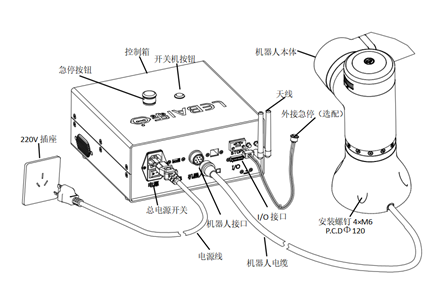
\includegraphics{image/1-2-host.png}
    \caption{机器人本体及控制箱连接}
    \label{fig:机器人本体及控制箱连接}
\end{figure}

\subsection{I/O接口}

LM3提供的I/O接口有两部分:控制箱和末端法兰盘,根据不同的应用场景,您可以选择不同位置的I/O接口来实现相应的I/O操作。

\begin{enumerate}
    \item 如\prettyref{fig:控制箱IO}和\prettyref{tab:控制箱IO},机器人控制箱提供:
    \begin{itemize}
        \item 4个数字输入,4个数字输出接口;
        \item 2个模拟输入,2个模拟输出接口。
    \end{itemize}

\begin{figure}[ht]
    \centering
    \includegraphics[height=4cm]{image/13.pdf}
    \caption{控制箱I/O硬件接口示意图}
    \label{fig:控制箱IO}
\end{figure}

\begin{table}[ht]
    \centering\small
\begin{tabular}{|c|c|l|}\hline
   \bf 序号	&  \bf 功能	& \bf  性能参数\\\hline
    1	&   电源正极	& $24\unit{V}$  \\\hline
    2	&   模拟输出1   &  \multirow{2}{5cm}{电压型:输出电压$0\sim 10\unit{V}$;\\电流型:输出电流$4\sim 20\unit{mA}$。
    }\\\cline{1-2}
    3	&   模拟输出2 & \\\hline
    4	&   数字输出1	&   \multirow{4}{5cm}{输出电压$24\unit{V}$,最大电流$2\unit{A}$。}\\\cline{1-2}
    5	&   数字输出2	&   \\\cline{1-2}
    6	&   数字输出3	&   \\\cline{1-2}
    7	&   数字输出4	&   \\\hline
    8	&   电源负极	&   \\\hline
    9	&   模拟输入1 &   \multirow{2}{5cm}{电压型:输出电压$0\sim 10\unit{V}$;\\电流型:输出电流$4\sim 20\unit{mA}$。
    }\\\cline{1-2}
    10	&   模拟输入2	&   \\\hline
    11	&   数字输入1	&   \multirow{4}{5cm}{输入电压$3\sim 30\unit{V}$。}\\\cline{1-2}
    12	&   数字输入2	&   \\\cline{1-2}
    13	&   数字输入3	&   \\\cline{1-2}
    14	&   数字输入4	&   \\\hline
    15	&   电源负极	   &     \\\hline
\end{tabular}
\caption{控制箱I/O接口引脚说明}
\label{tab:控制箱IO}
\end{table}
\clearpage
    \item 如\prettyref{fig:法兰盘IO}和\prettyref{tab:法兰盘IO},末端法兰盘上提供:
    \begin{itemize}
        \item 2个数字输入接口;
        \item 2个数字输出接口。
    \end{itemize}

\begin{figure}[ht]
    \centering
    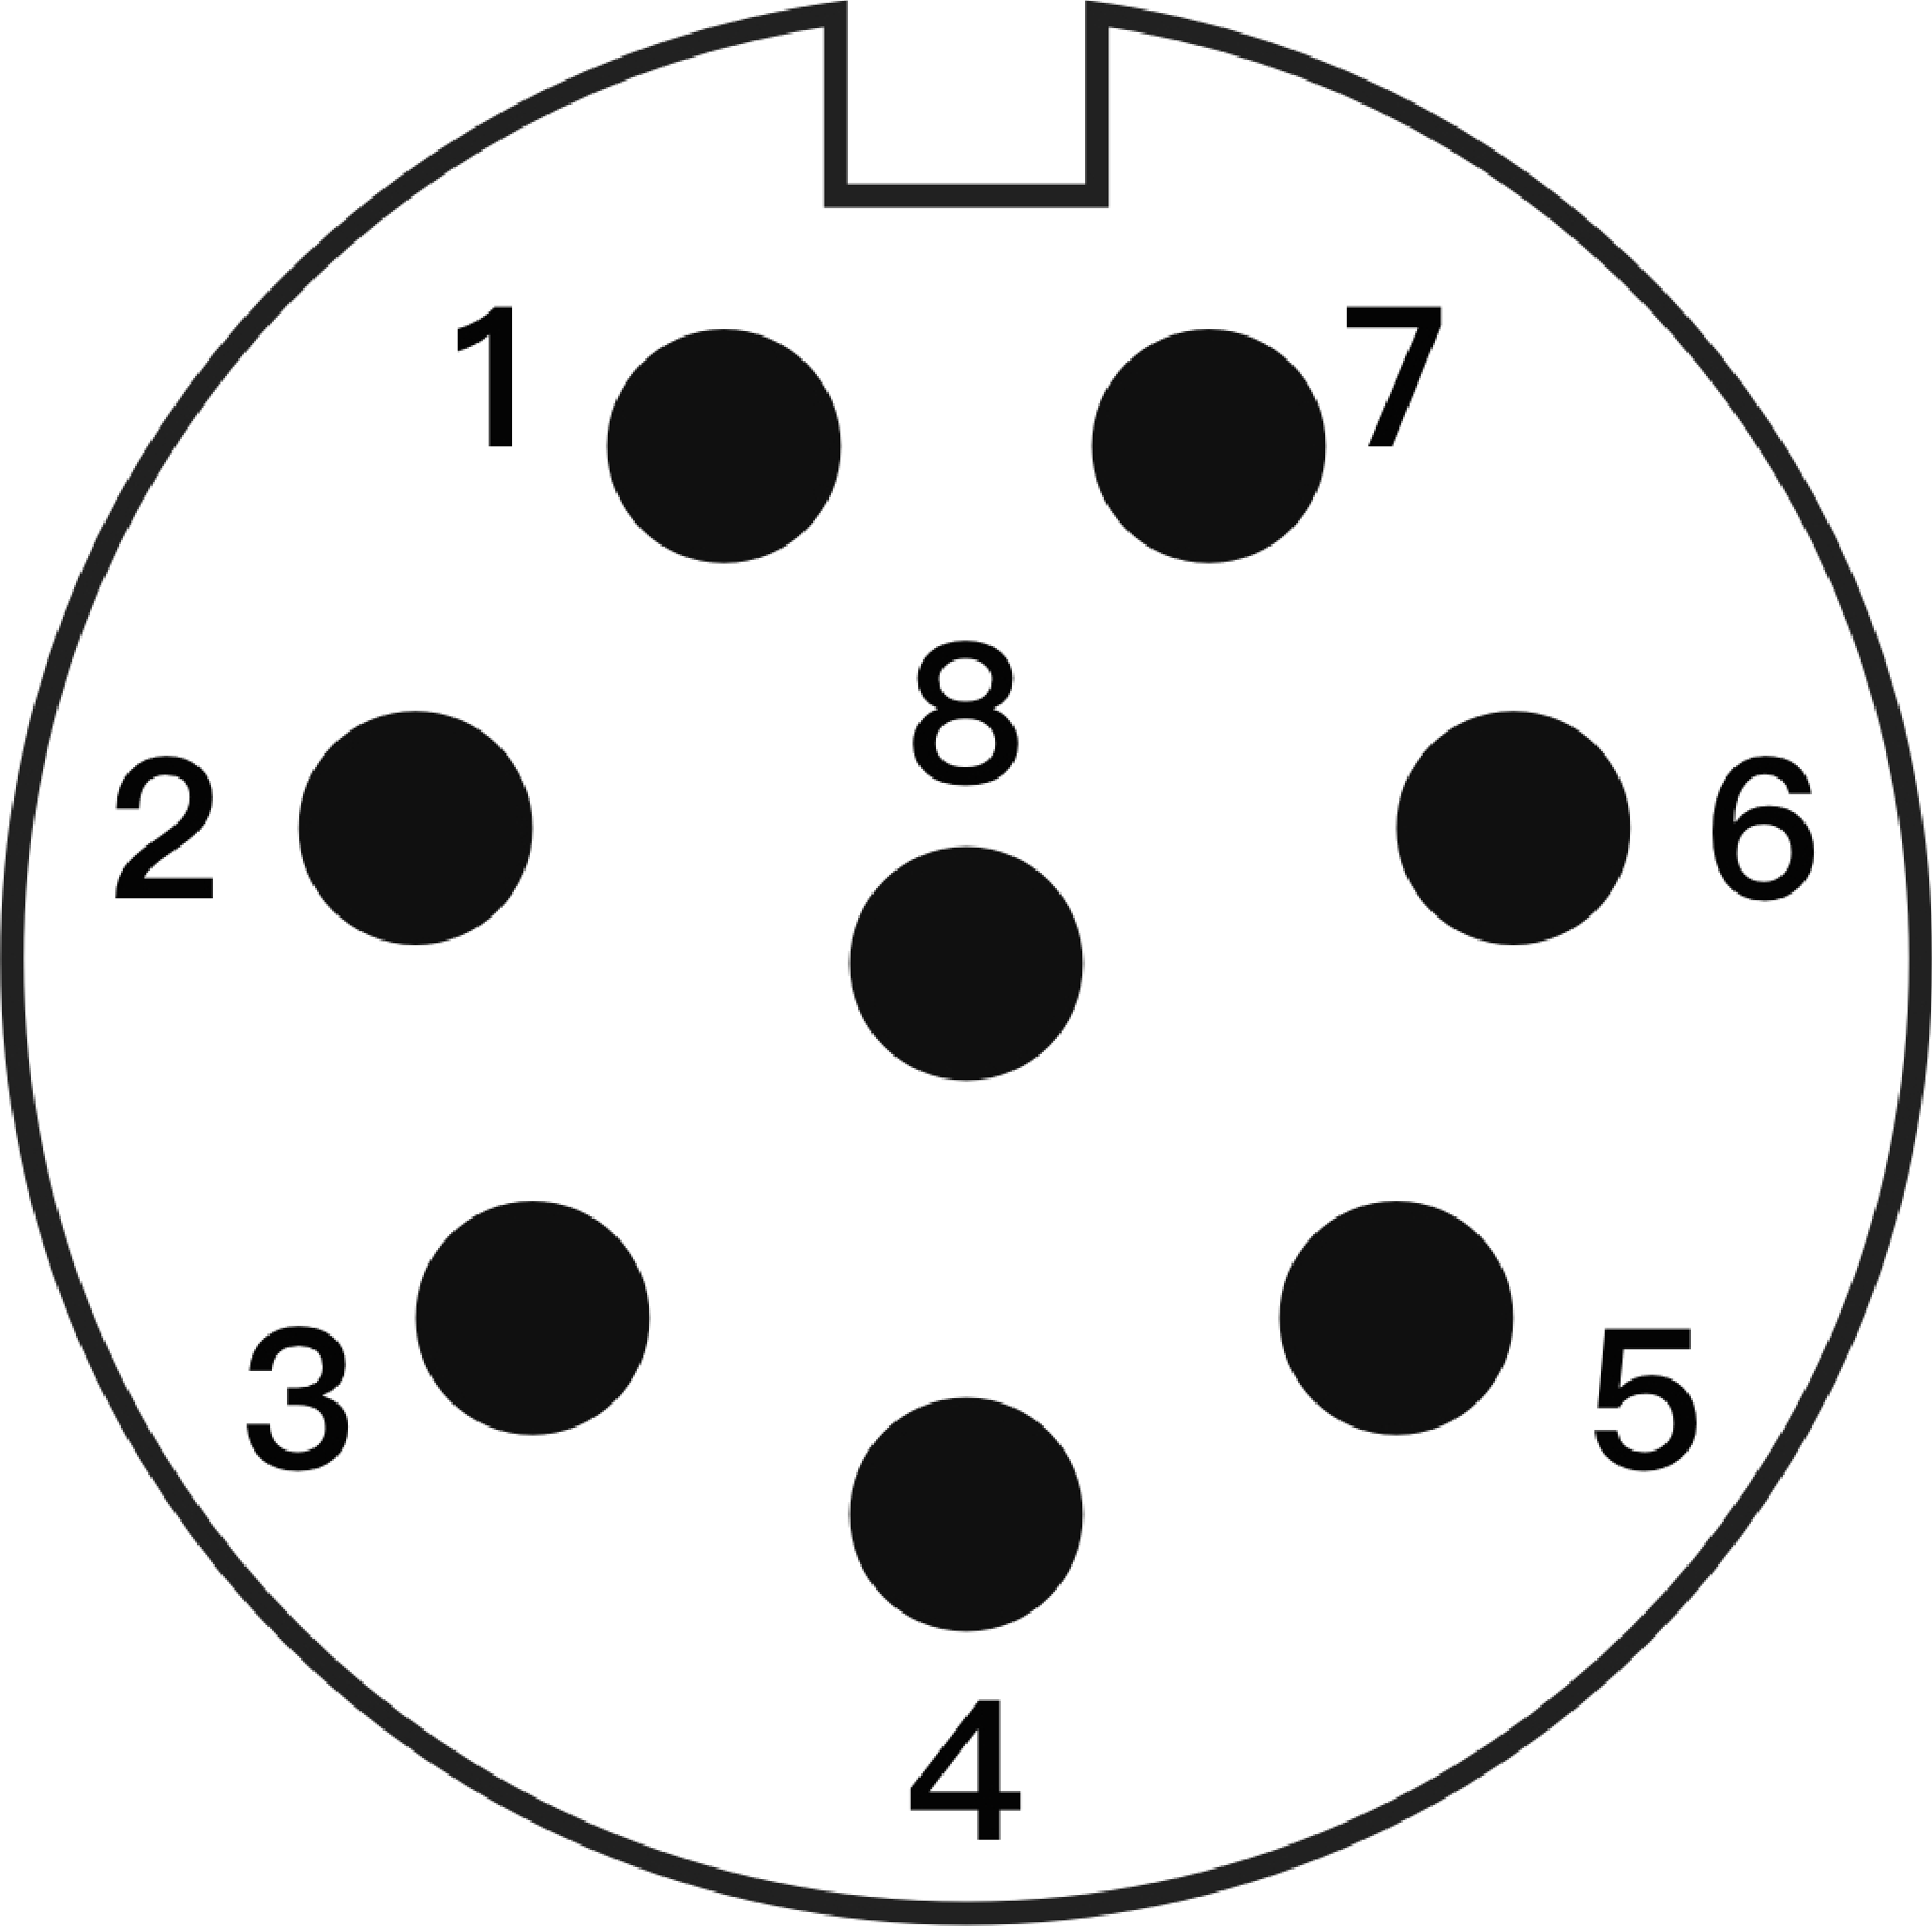
\includegraphics[height=2cm]{image/35.pdf}
    \caption{末端法兰盘 I/O硬件接口示意图}
    \label{fig:法兰盘IO}
\end{figure}

\begin{table}[ht]
    \centering\small
\begin{tabular}{|c|c|l|}\hline
   \bf 序号	&  \bf 功能	& \bf  性能参数\\\hline
    1	&   电源正极   &  \multirow{2}{5cm}{
            电压$24\unit{V}$,最大电流$2\unit{A}$。
    }\\\cline{1-2}
    2	&   电源负极 & \\\hline
    3	&   数字输出1	&   \multirow{2}{5cm}{输出电压$24\unit{V}$,最大电流$2\unit{A}$。}\\\cline{1-2}
    4	&   数字输出2	&   \\\hline
    5	&   CANH	&   \\\hline
    6	&   CANL	&   \\\hline
    7	&   数字输入1	&   \multirow{2}{5cm}{
            输入电压$3\sim 30\unit{V}$。
    }\\\cline{1-2}
    8	&   数字输入2	&   \\\hline
\end{tabular}
\caption{末端法兰盘I/O引脚说明}
\label{tab:法兰盘IO}
\end{table}

\end{enumerate}

\section{机器人安装}

如\prettyref{fig:机器人安装方式},LM3机器人支持三种安装方式:正装、倒装、侧装(侧装时注意机器人电缆出口必须朝下)。使用机器人配件包中的 4 颗 M6 螺钉,对应机器人底座上的 4 个安装孔进行安装操作,建议以 $9\Nm$ 扭矩紧固这些螺钉。如果需要更准确地调整机器人位置,还可钻2 个直径$5 \mm$的孔,并用销加以固定。

\begin{figure}[ht]
    \centering
    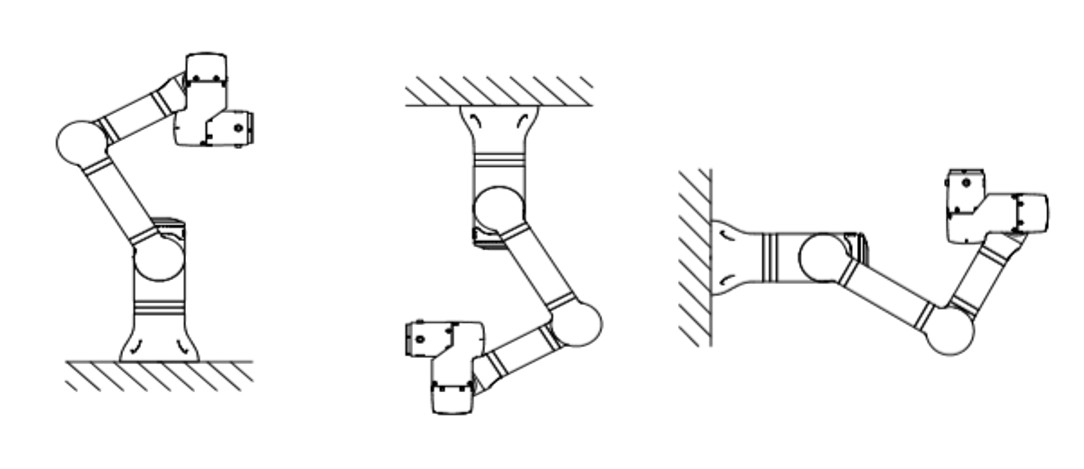
\includegraphics[width=\textwidth]{image/1-4-direction.jpg}
    \caption{机器人安装方式}
    \label{fig:机器人安装方式}
\end{figure}

 
\begin{figure}[ht]
    \centering
    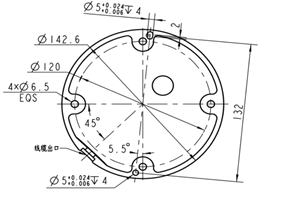
\includegraphics{image/1-5-base.png}
    \caption{机器人底座视图}
    \label{fig:机器人底座视图}
\end{figure}


\info{机器人每一个安装孔位都应固定螺钉,固定后的每个螺钉都应能提供最小抗倾覆力;\\
机器人安装时,应扶住机器人直至底座所有螺钉全部紧固好。
}

\danger[警告]{切勿将机器(含机箱)固定在不稳固的位置,否则可能会跌落损坏。}
 % 2	准备工作
\chapter{基础操作}
\label{cha:基础操作}

\section{机器人上电}

操作前,请再次确认已阅读并确保已遵循\prettyref{sec:安全指南}内容,排除潜在风险,确保操作安全。

\begin{figure}[hb]
    \centering
    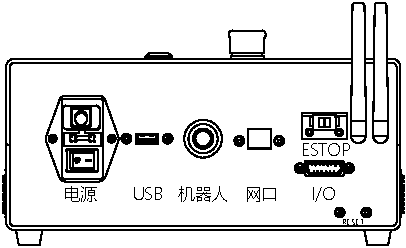
\includegraphics[height=4cm]{line_graphs/robot_control_box_back.pdf}
    \caption{控制箱背板示意图}
    \label{fig:控制箱背板示意图}
\end{figure}

\begin{enumerate}
\item 将机器人电缆插头插入控制箱的机器人接口;
\item 控制箱插上电源线,并将电源插头接入$220 \unit{V}$交流电插座;
\item 确保控制箱顶部的急停按钮处于释放\footnote{当机器按钮处于弹起状态时为释放状态,反之处于按下状态为锁定状态。}状态;
\item 打开控制箱背板的红色总电源开关,开关指示灯亮;
\item 长按控制箱顶部的开关机按钮(约3 秒),直至蓝色灯光常亮,等待机器人肩部灯光亮起,完成控制箱和机器人的上电操作。
\end{enumerate}

\danger{\begin{itemize}
\item 请确保控制箱电源的插线板务必良好接地;
\item 请确保控制箱电源的输入电流受到漏电保护装置和适当的过流断路保护装置的保护;
\item 请确保所有的电缆在控制箱通电前都正确连接,始终正确使用原装的电源线。
\end{itemize}}

\danger[警告]{\begin{itemize}
\item 禁止在机器人启动时断开或用力拉拽机器人电缆;
\item 禁止延长或改动机器人电缆;
\item 切勿损坏电源线,或将重物压在电源线上;
\item 切勿使用破损或不符合的插座。
\item 切勿让电源插头和插座粘附灰尘和金属附着物。
\end{itemize}}

\clearpage

\section{连接机器人}
LM3支持有线网络连接和无线网络连接,无线网络连接目前仅支持接入控制箱内置的Wi-Fi热点网络。
\subsection{有线网络连接}

使用网线将控制箱背板的网口与路由器或交换机连接,同时确保用于操作机器人的电脑、平板、手机或其他图形化终端设备与机器人接入的是同一网络。

有线网络的连接示意如\prettyref{fig:有线网络连接拓扑图}:

\begin{figure}[ht]
    \centering
    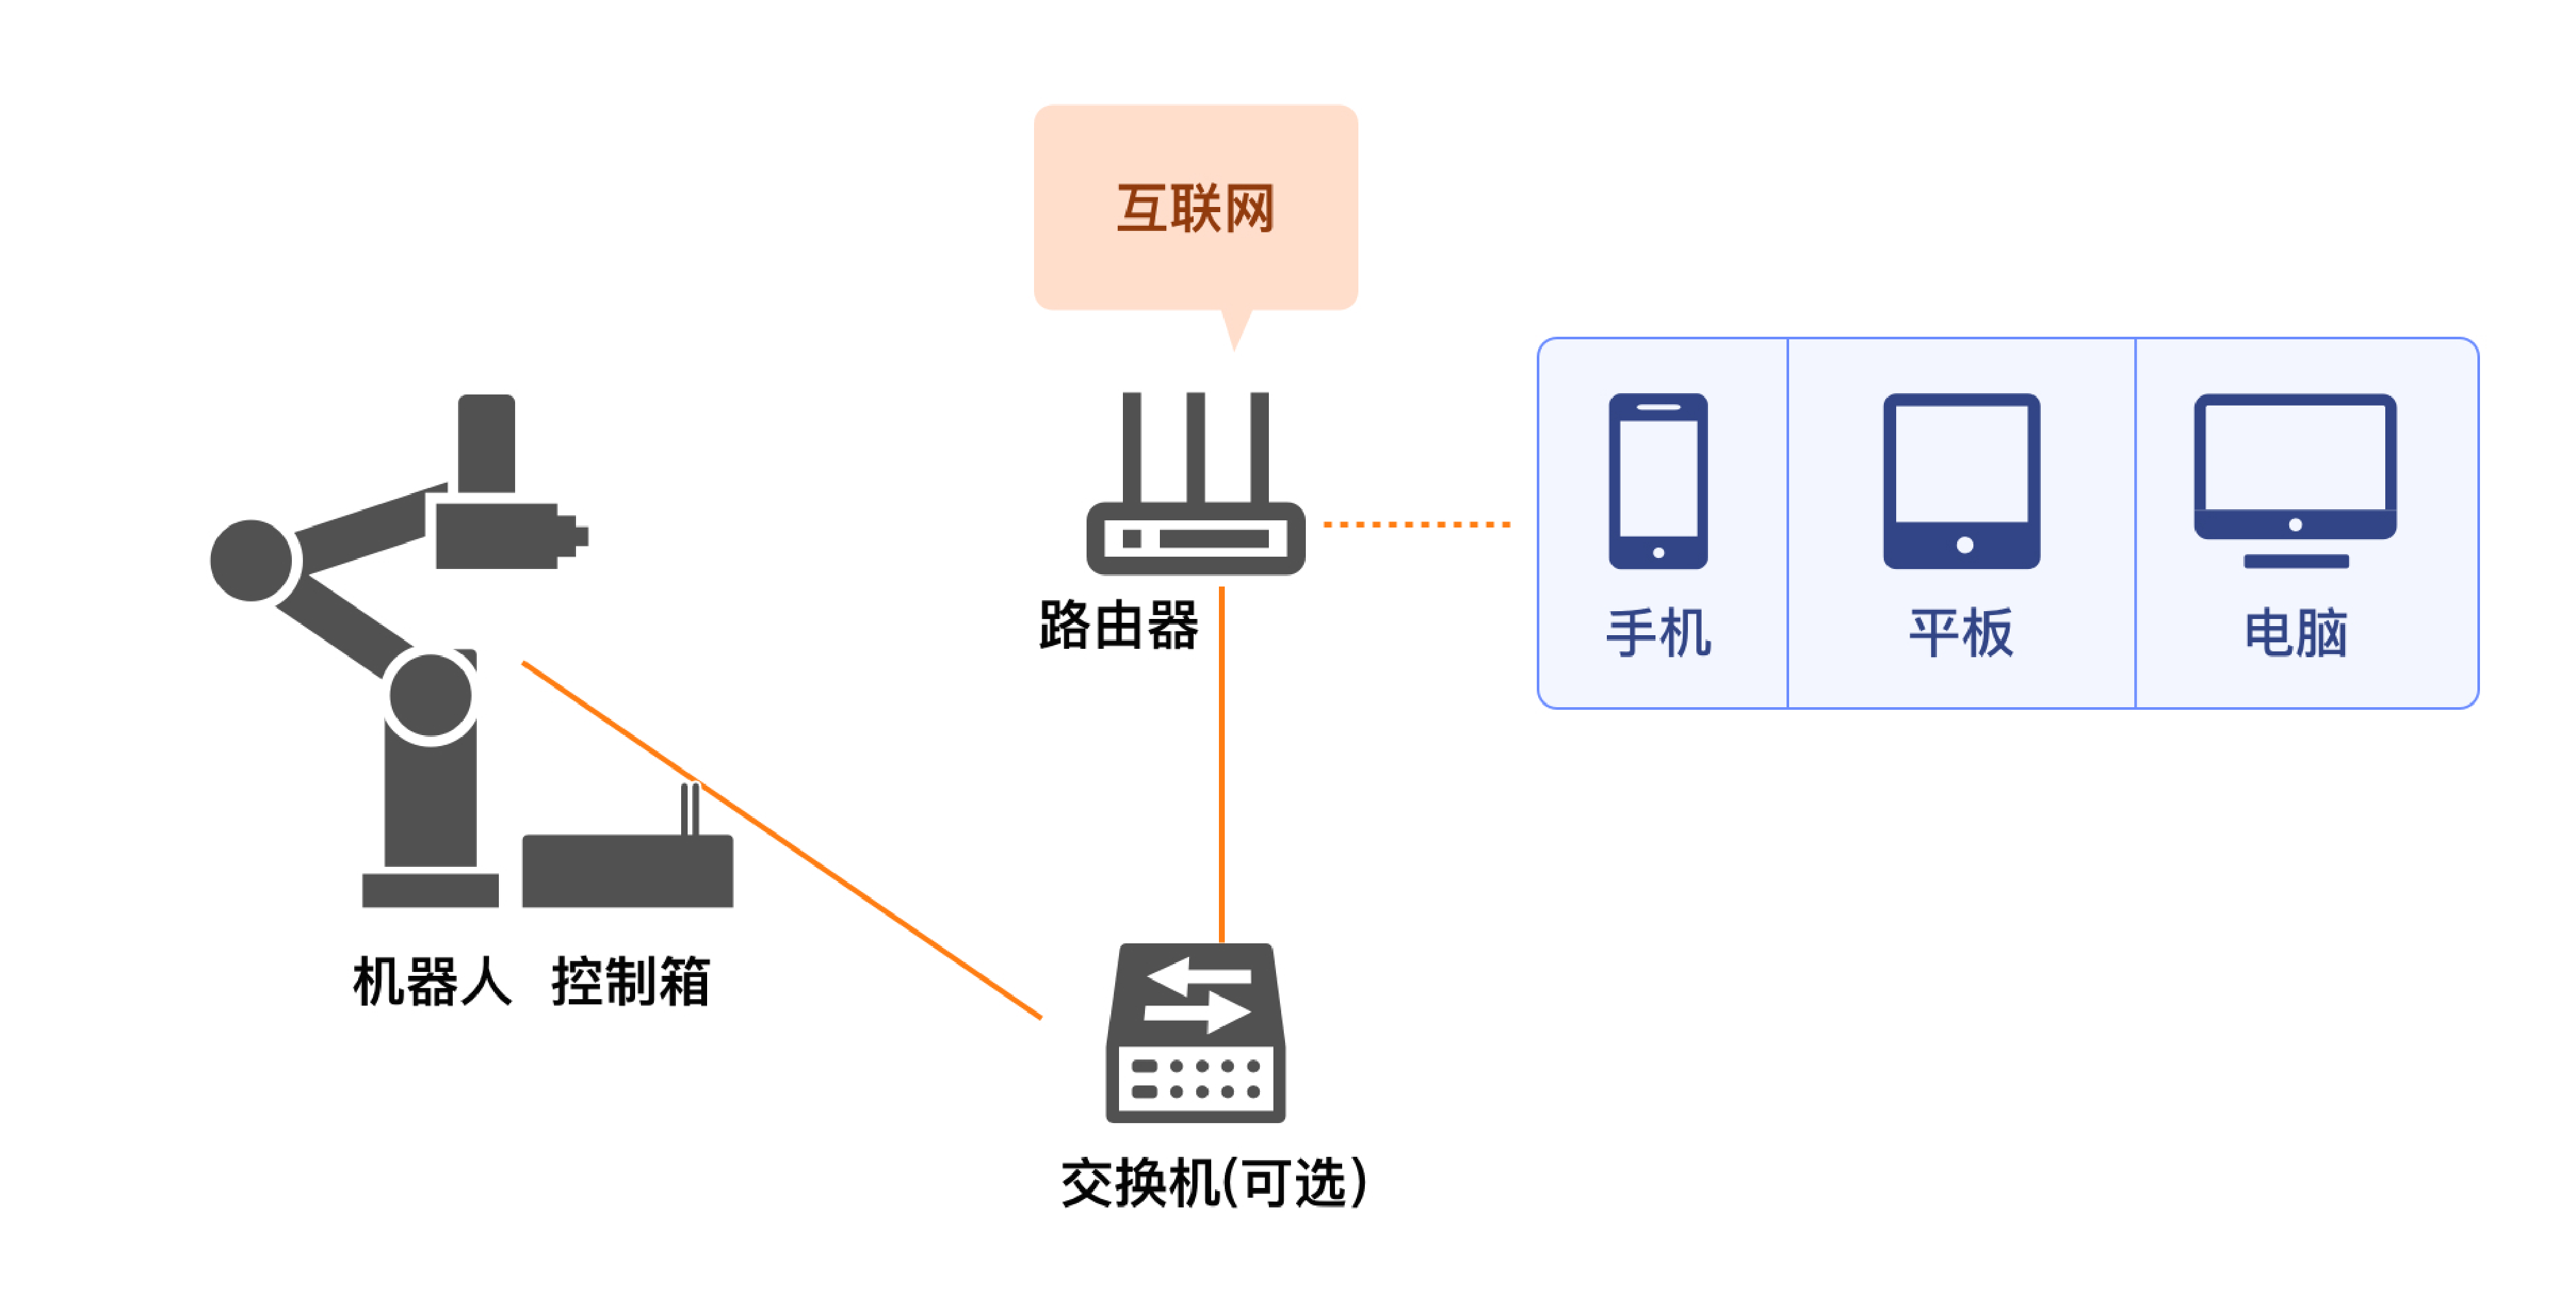
\includegraphics[width=\textwidth]{image/1103/5.pdf}
    \caption{有线网络连接拓扑图}
    \label{fig:有线网络连接拓扑图}
\end{figure}

\clearpage

\subsection{无线网络连接}
机器人出厂后,默认会启用一个热点名称为设备名称  的Wi-Fi热点,设备名称格式如:\verb|Lebai-123456|(后6位为随机字符),默认密码为:\verb|88888888|(8个8)。可通过电脑、平板、手机或其他图形化终端设备的Wi-Fi功能连接该设备名称对应的Wi-Fi热点网络,连接和控制机器人。

\begin{figure}[ht]
    \centering
    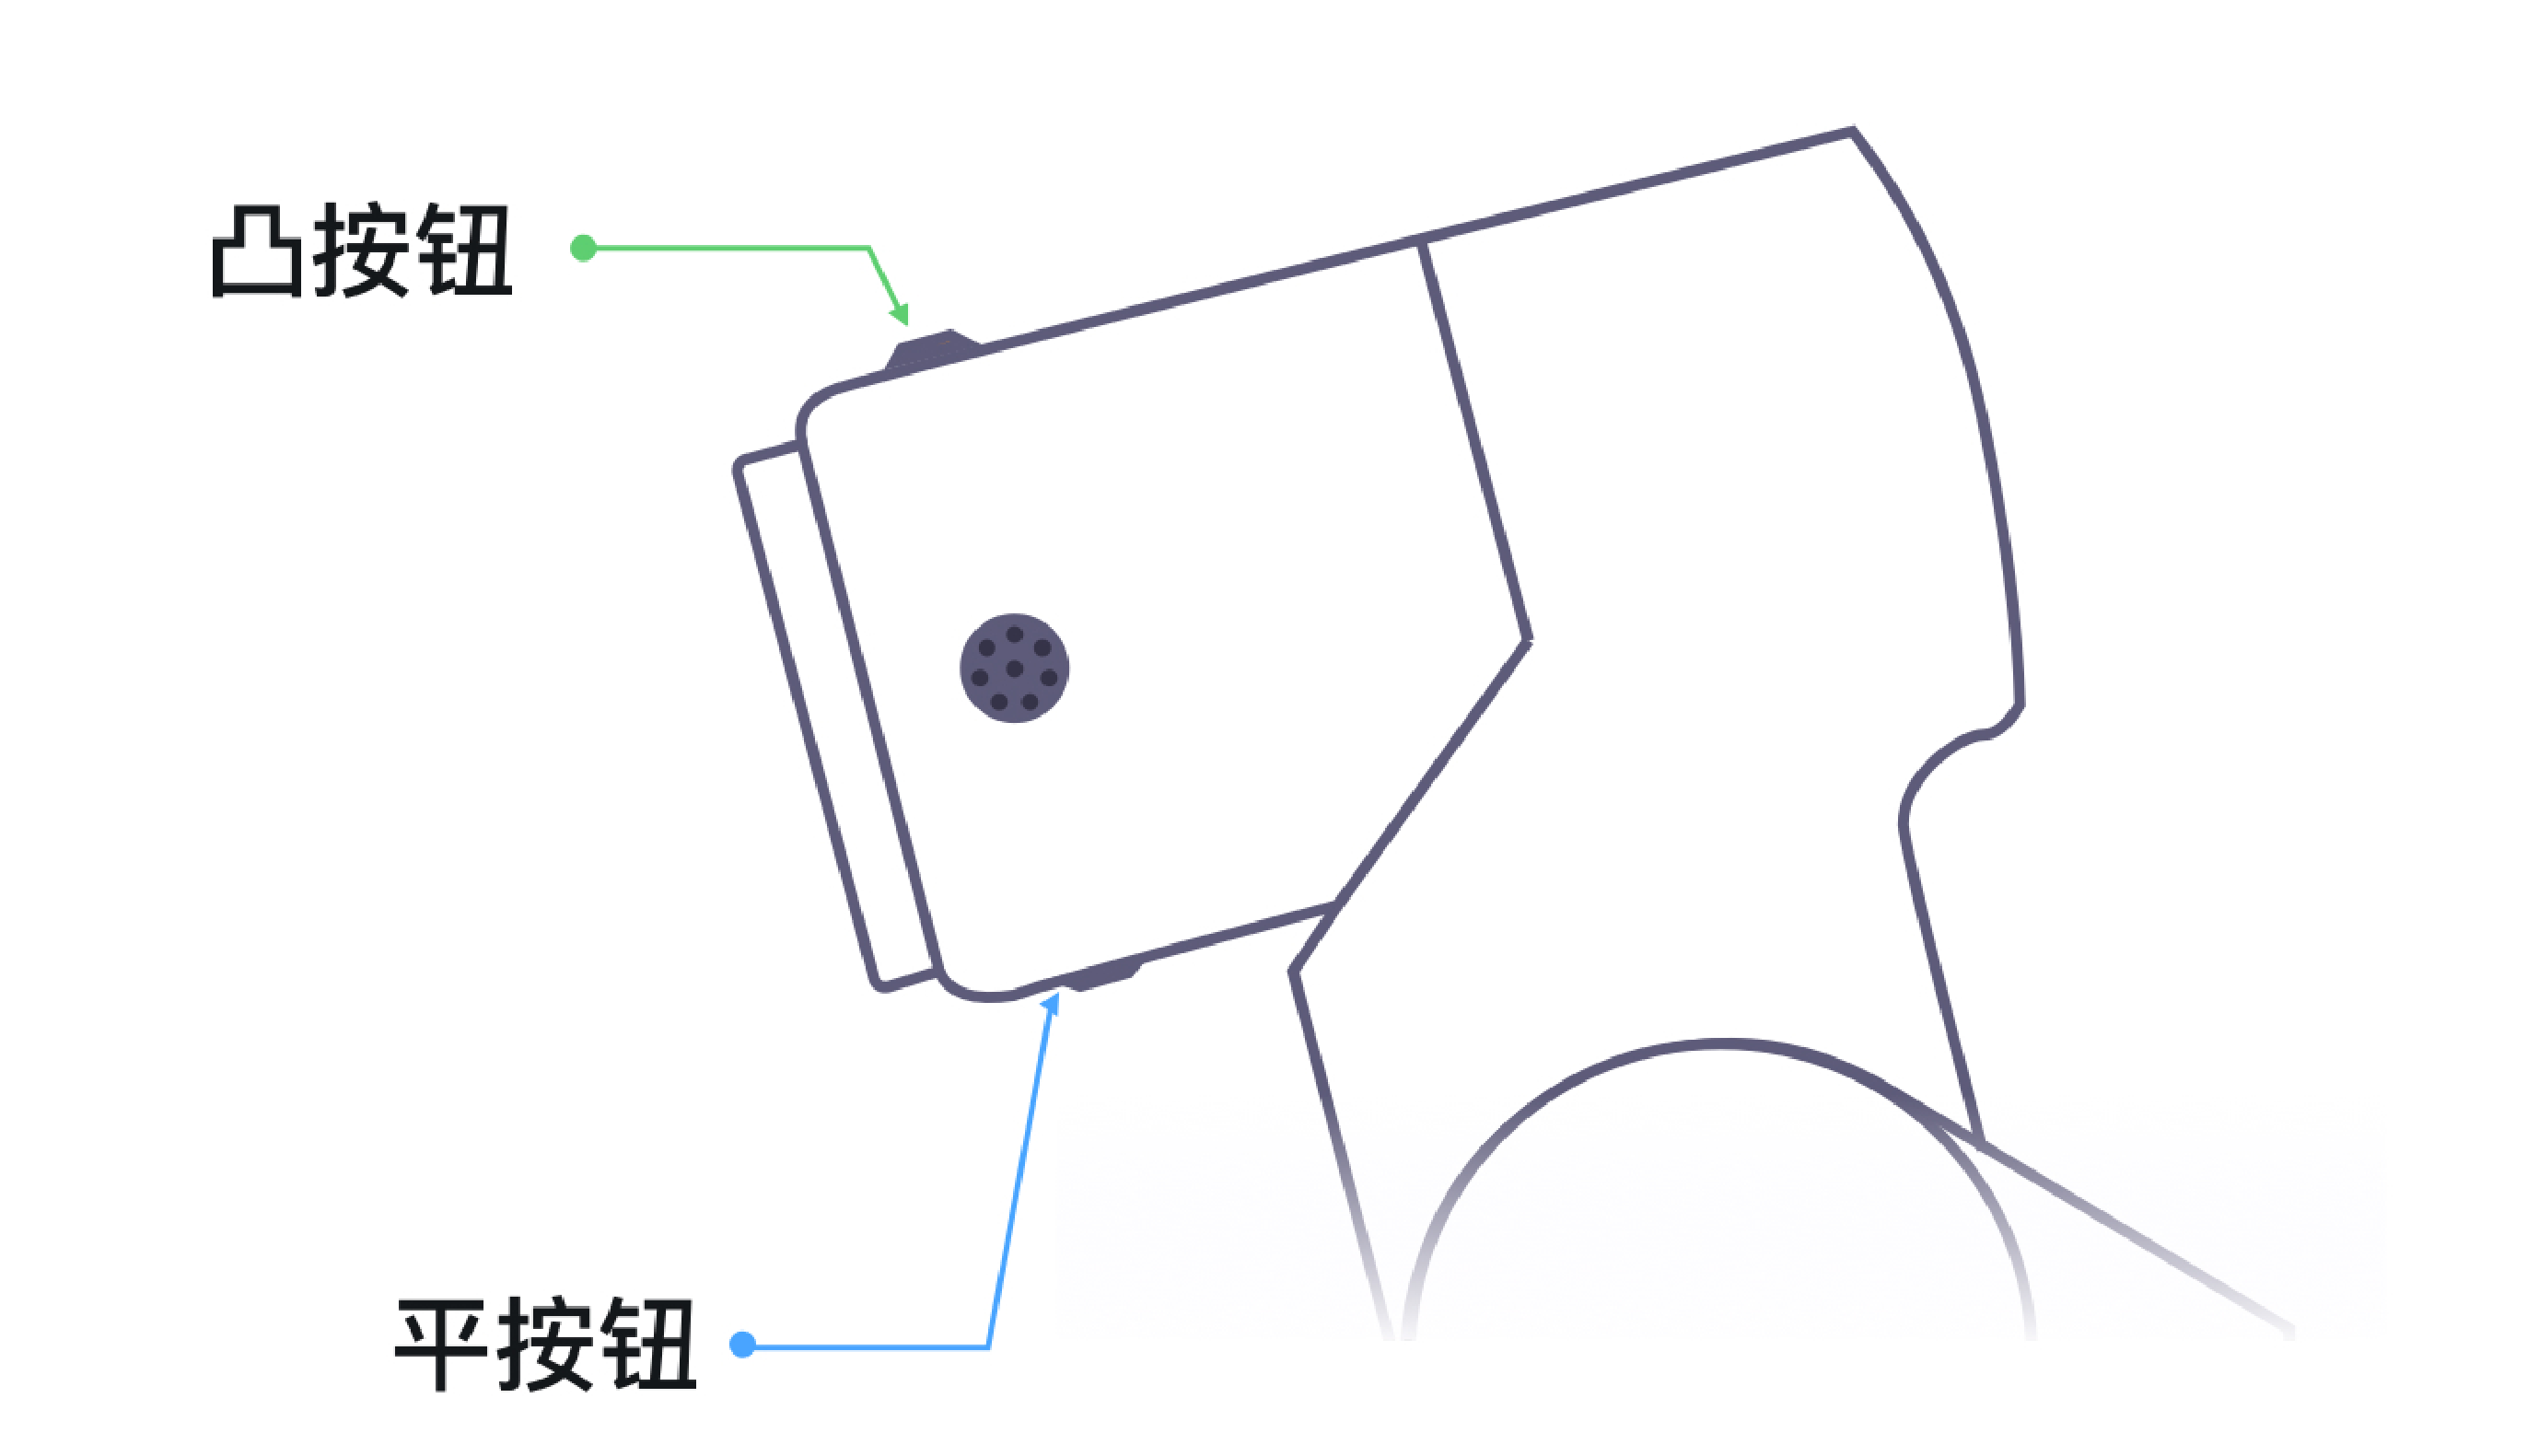
\includegraphics[width=\textwidth]{image/12.pdf}
    \caption{无线网络连接拓扑图}
    \label{fig:无线网络连接拓扑图}
\end{figure}

\clearpage

\section{登录\LM}
熟悉\LM 系统的操作将有助于您更方便和快速地上手使用本公司的机器人产品。
打开电脑、平板、手机或其他图形化终端设备的浏览器,在地址栏输入如下地址:
\begin{itemize}
	\item 若使用有线网络,地址\footnote{有线网络地址在接入的网络路由器页面中的设备列表里查看,查看方式因设备品牌和类型的不同而有差异,具体查看方式请参考路由器设备的说明书或联系对应设备厂商。}为:\url{http://<IP>}
	\item 若使用无线热点,地址为:\url{http://10.20.17.1}
\end{itemize}

网页打开后会进入登录页面,请输入默认授权码:\verb|1111|,点击\btn{登录}或按\kbd{Enter},登录\LM。

\begin{figure}[ht]
    \centering
    
\includegraphics[width=0.8\textwidth]{screen/2-4.png}
    \caption{登录\LM}
    \label{fig:登录LM}
\end{figure}

\clearpage

\section{设置引导页}

当机器人开箱上电后,第一次登录\LM 时,首先需要按照设置引导页的提示进行初次使用的安装设置。
\subsection{系统设置}
在此步可以自定义语言、时区、时间。

\begin{figure}[ht]
    \centering
    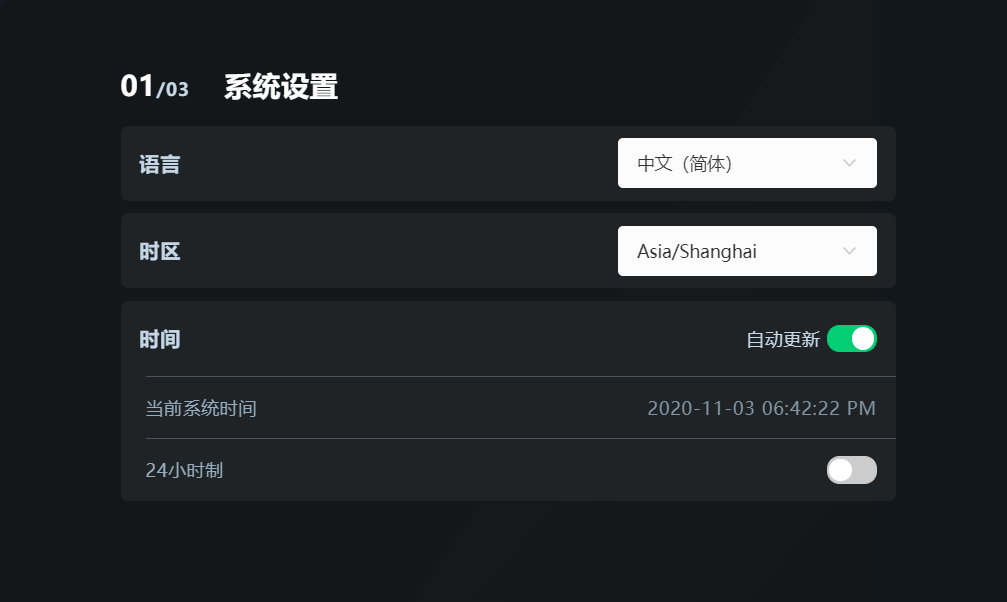
\includegraphics[width=\textwidth]{screen/2-5.png}
    \caption{系统设置}
    \label{fig:系统设置}
\end{figure}

\subsection{机器人设置}
在此步中可以设置机器人的安装方式、操作模式及碰撞检测。
\begin{enumerate}
\item 安装方式

	根据实际安装方式,参照\prettyref{fig:安装方式}中的“图标对照表”选择正装、倒装、侧装。

	\begin{figure}[ht]
		\centering
		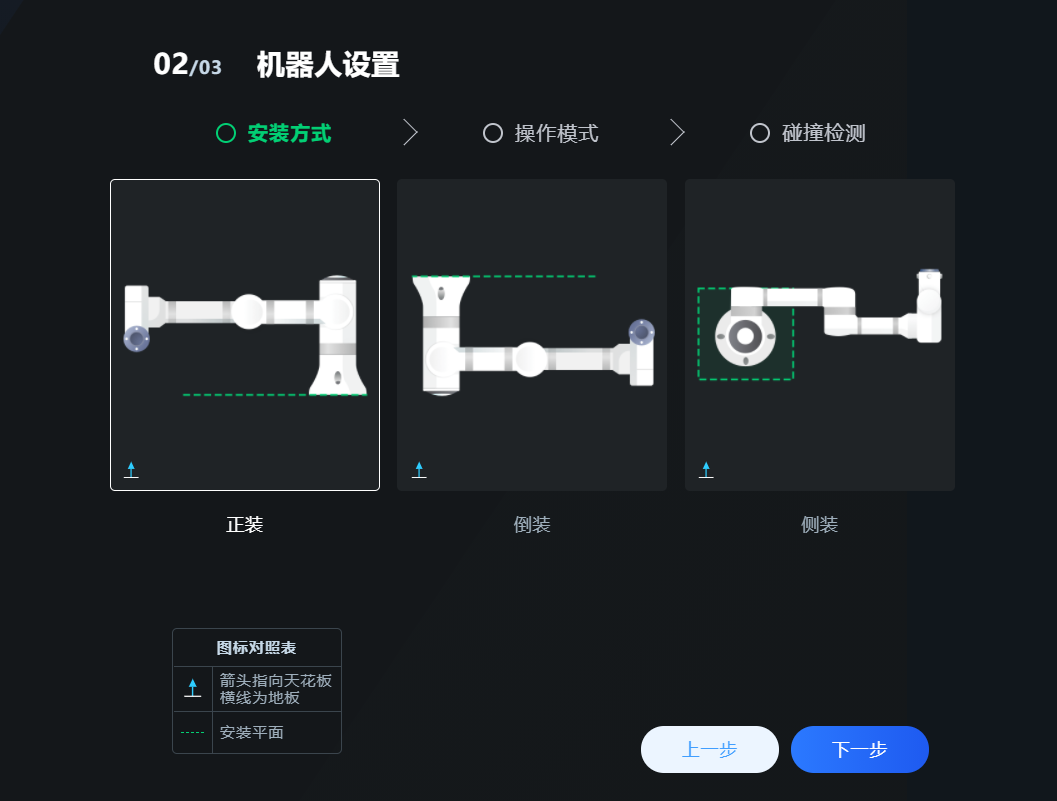
\includegraphics[width=\textwidth]{screen/2-6.png}
		\caption{安装方式}
		\label{fig:安装方式}
	\end{figure}

	\danger{安装方式的选择一定要与实际安装方式一致,否则有可能导致误伤。}

\clearpage

\item 操作模式

	可在新手模式、专家模式中选择。新手模式适合没有编程基础的新手,无需理解任何逻辑和代码;专家模式适合有一定编程基础和逻辑基础的高级用户,您可以根据自身情况选择相应的操作模式。

	\begin{figure}[ht]
		\centering
		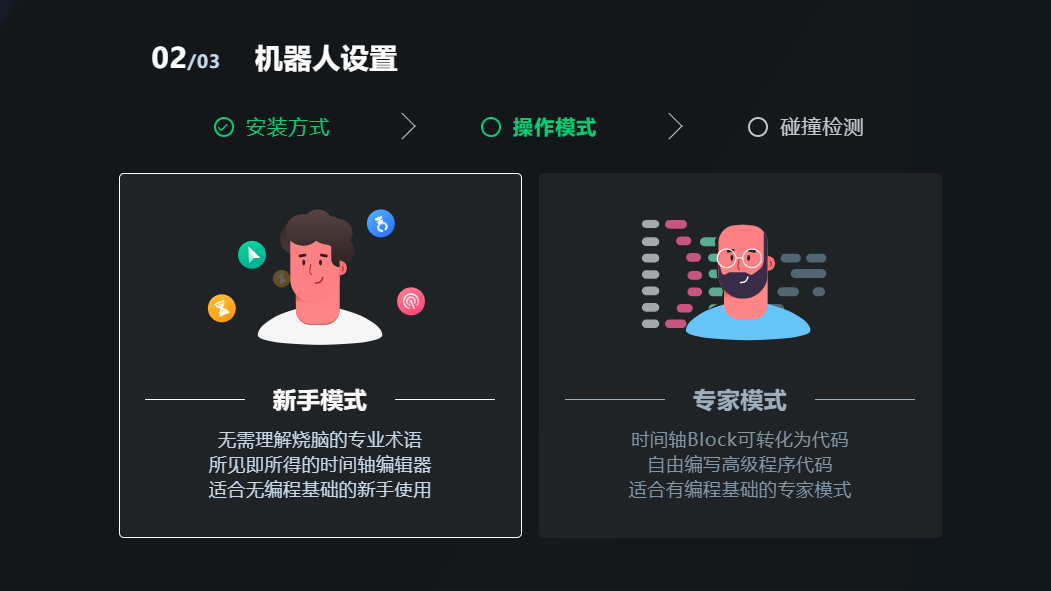
\includegraphics[width=\textwidth]{screen/2-7.png}
		\caption{操作模式}
		\label{fig:操作模式}
	\end{figure}

\clearpage

\item 碰撞检测

	检测开关默认为开,“碰撞后的动作”默认为\mnu{急停},可选择\mnu{急停}或\mnu{暂停},同时可以拖动拉杆来调整“检测灵敏度”大小。点击\btn{下一步},进入界面设置。

	\begin{figure}[ht]
		\centering
		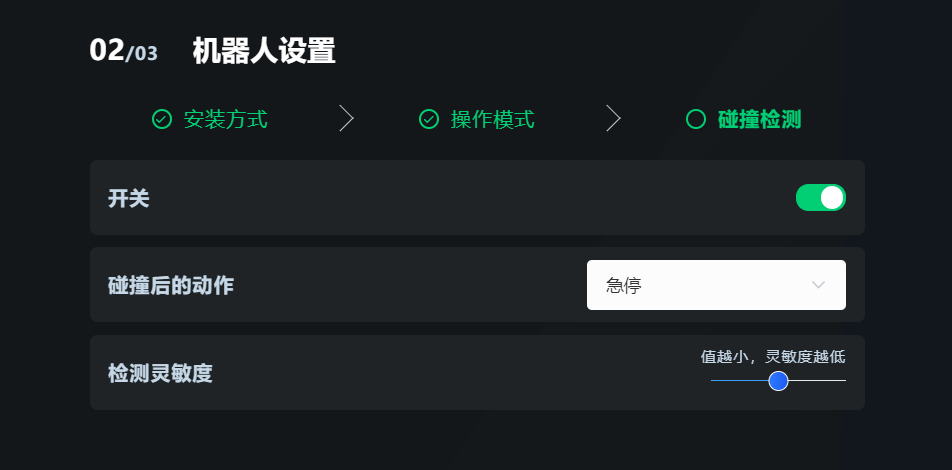
\includegraphics[width=\textwidth]{screen/2-8.png}
		\caption{碰撞检测}
		\label{fig:碰撞检测}
	\end{figure}

	\danger{机器人运行过程中,无论是否开启“碰撞检测”功能,禁止在没有防护的情况下进入到机器人作业半径范围内,否则存在人员被机器人撞伤,卷入的危险。}

\end{enumerate}

\clearpage

\subsection{界面设置}

在界面设置中,建议您选择使用\mnu{深色主题}。
% 可以选择\mnu{深色主题}或\mnu{浅色主题},目前\LM 浅色主题还在测试阶段,

\begin{figure}[ht]
	\centering
	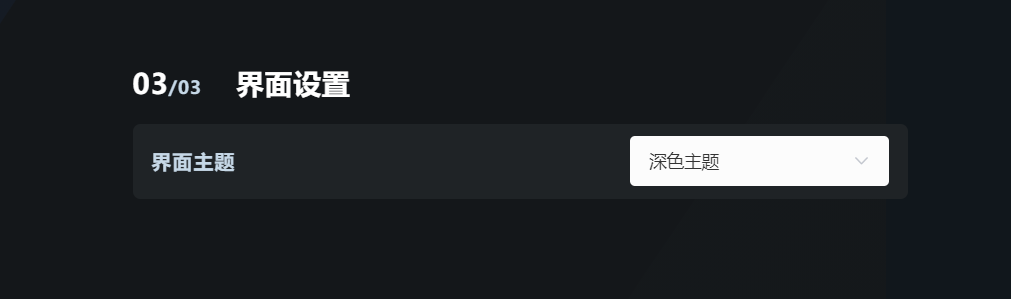
\includegraphics[width=\textwidth]{screen/2-9.png}
	\caption{界面设置}
	\label{fig:界面设置}
\end{figure}

点击\btn{完成},进入\LM 首页。

\clearpage

\section{首页}

在\LM 首页,页面分为:左面板、状态区、控制区、主功能入口、任务历史以及顶部标题栏六个区域。

左面板显示机器人整机温度及关节温度数据,坐标空间的位置和姿态数据,关节空间的关节角度数据;状态区显示机器人的实时状态;控制区包含机器人的启停按钮,软件示教按钮以及速度比例调整控件;主功能入口包含场景、控制和设备三个主功能入口;任务历史包含所有的任务历史列表;顶部标题栏右侧包含设置、消息中心和退出登录。

\begin{figure}[ht]
	\centering
	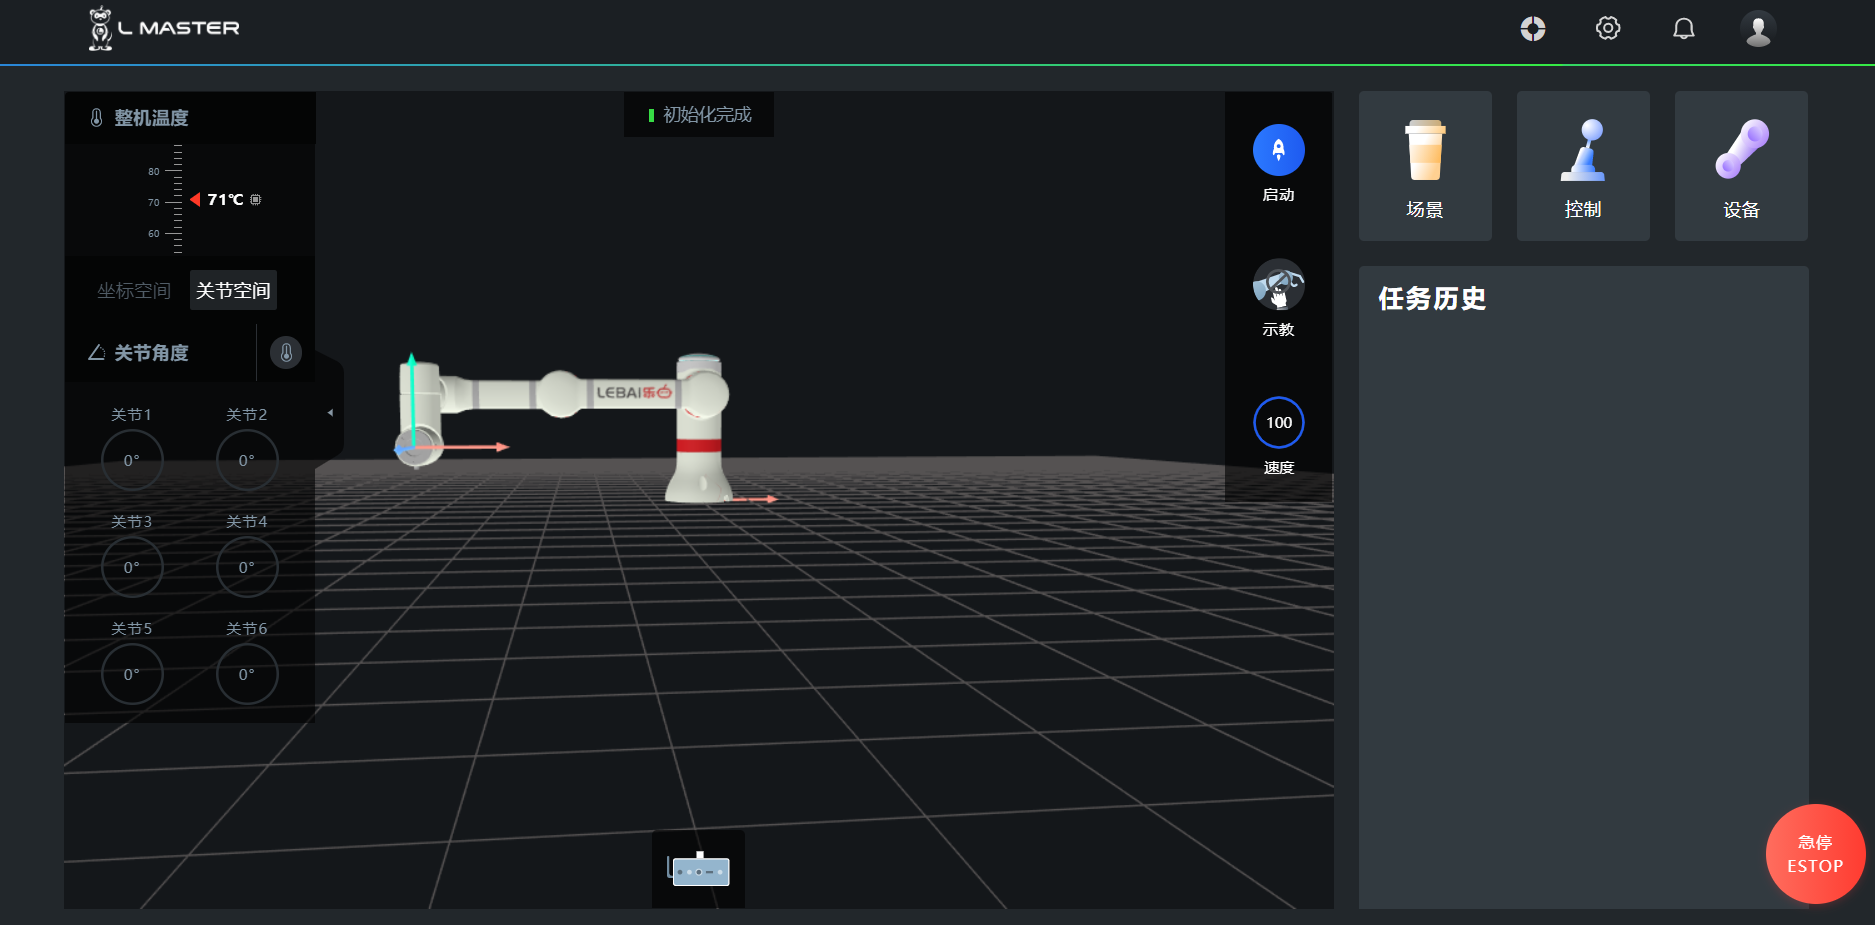
\includegraphics[width=\textwidth]{screen/2-10.png}
	\caption{\LM 首页}
	\label{fig:LM首页}
\end{figure}

\clearpage

\subsection{机器人状态}

机器人状态区显示机器人当前状态,具体说明可参考\prettyref{tab:机器人状态列表}。

\begin{table}[ht]
    \centering\small
    \begin{tabular}{|l|l|}\hline
\sf 状态 & \sf 说明\\\hline
硬件通讯故障 & 机器人通讯故障或控制系统异常\\\hline
已急停,请确认安全性 & 机器人处于急停状态\\\hline
初始化中 & 机器人初始化中\\\hline
初始化完成 & 机器人电源已开启\\\hline
空闲 & 机器人处于空闲状态\\\hline
运行中 & 机器人运行中\\\hline
更新中 & 机器人系统更新中\\\hline
启动中 & 机器人初始化完成到空闲的启动过程中\\\hline
正在停止 & 机器人空闲状态转到停止状态\\\hline
示教中 & 机器人处于示教模式中\\\hline
已停止 & 机器人处于停止状态,非急停状态\\\hline
    \end{tabular}
    \caption{机器人状态列表}
    \label{tab:机器人状态列表}
\end{table}

\subsection{温度}
如\prettyref{fig:温度信息},\LM 首页左上方实时监测机器人整机温度\footnote{整机温度:取控制箱内控制器的CPU温度和机器人每个关节的温度的最大值作为整机温度的显示,当整机温度数值右侧显示芯片图标为表示当前CPU温度值最高,显示一个关节加数字图标时表示该数字对应的关节温度较高。},每个关节正常温度范围值在室温至65 ℃之间。点击左边区域的关节空间标签中关节角度的右侧温度计图标,可实时观测关节1至关节6的温度变化;再次点击该图标,可以切换回关节角度显示。

\danger[警告]{当关节温度显示超过65℃时,请勿触摸机器外表面,否则有高温烫伤风险,并请立即停机,待机器温度回到常温,再检查当前机器人负载是否超过额定有效负载$3\kg$或者机器人是否碰撞到外部物品。}

\begin{figure}[ht]
	\centering
	\begin{minipage}[t]{0.32\linewidth}
		\centering
		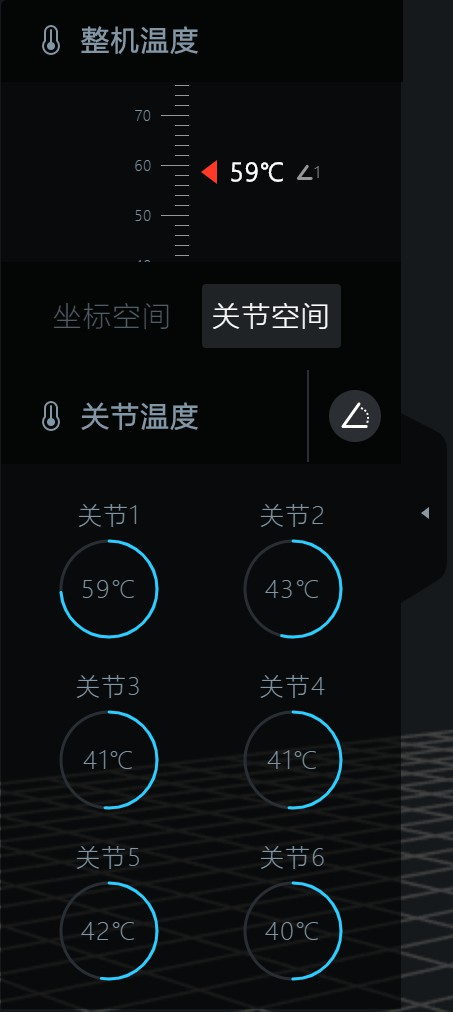
\includegraphics[height=6cm]{screen/2-11-t.jpg}
		\caption{关节温度}
		\label{fig:温度信息}
	\end{minipage}
	\begin{minipage}[t]{0.32\linewidth}
		\centering
		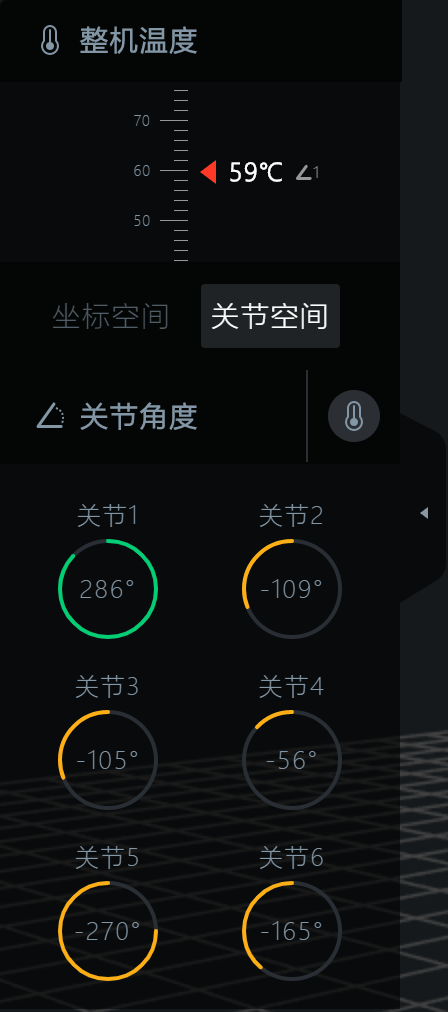
\includegraphics[height=6cm]{screen/2-12-1.png}
		\caption{关节空间}
		\label{fig:关节位置信息}
	\end{minipage}
	\begin{minipage}[t]{0.32\linewidth}
		\centering
		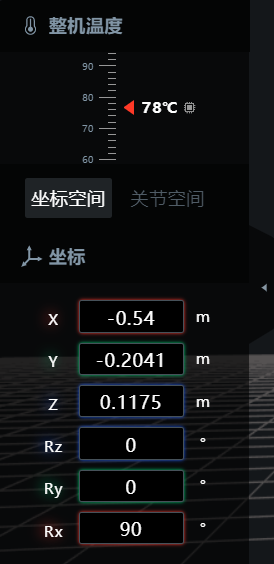
\includegraphics[height=6cm]{screen/2-12.png}
		\caption{坐标空间}
		\label{fig:坐标位置信息}
	\end{minipage}
\end{figure}

\subsection{位置信息}
\LM 首页左侧区域实时同步机器人位置信息,包含坐标空间和关节空间。如\prettyref{fig:坐标位置信息},坐标空间显示机器人在坐标空间的位置和姿态的实时数据;如\prettyref{fig:关节位置信息},关节空间显示机器人6个关节角度的实时数据。

\subsection{速度因子}
点击\LM 首页示教按钮下方的速度图标,在展开的滑动条中拖动滑块或点击滑动条以调整机器人的运行速度比例,调整区间为$0\sim 100$。

\begin{figure}[ht]
	\centering
	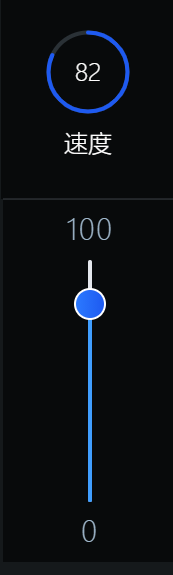
\includegraphics[height=4cm]{screen/2-13.png}
	\caption{速度因子}
	\label{fig:速度因子}
\end{figure}

\subsection{消息中心}
在消息中心中,可查看机器人提示、警告、软硬件异常的消息通知。鼠标移动到\LM 首页右上角的消息图标\icn[Black]{image/22.pdf}可以打开消息中心。

在消息中心中,有以下两种方式进行消息搜索:
\begin{enumerate}
	\item 通过关键字搜索消息通知;
	\item 通过筛选5种类型的机器人消息通知:
	\begin{description}
\item[\icn{image/30.pdf} 调试]
\item[\icn{image/29.pdf} 信息] 信息提醒类消息
\item[\icn{image/28.pdf} 警告] 系统运行时的警告级别的提醒,一般不影响使用
\item[\icn{image/27.pdf} 错误] 系统出现了错误,需要保持关注错误的发生概率,如果频繁发生需尽快点击查看解决方案或与本公司及时取得联系
\item[\icn{image/26.pdf} 致命] 系统出现严重错误,存在运行风险或已无法正常运行,此时必须立即停机查看解决方案或与本公司及时取得联系。
	\end{description}
\end{enumerate}

点击消息项的错误码链接,可跳转至本公司官网对应的错误码解决方案查看页面,在页面中可根据错误码查找对应的问题及解决方案。

\subsection{任务历史}
\label{sec:任务历史}
任务历史列表中显示正在运行中及已完成的任务,并以时间顺序排列展现。当任务正在运行时,任务历史标题栏会出现停止、暂停或恢复的控制按键。任务历史列表中:
\begin{itemize}
	\item 正在运行的任务右侧显示当前已运行次数;
	\item 已完成的任务右侧显示“重新运行”小旗帜\icn{image/38},点击可重新运行当前选择的任务。
\end{itemize}

点击“任务历史”列表项任务名称,进入该任务对应的场景编辑页面。

\danger[警告]{当运行某个场景,该场景的任务进入任务历史列表。该任务运行完成,点击“重新运行”按钮后,当前执行的任务为之前执行该任务的场景数据,即使该场景在该任务运行完后发生变更,也不会影响该任务的重新运行,重新运行的任务不受该场景的数据变更影响,以上一次运行任务的场景数据为准。}

\begin{figure}[htb]
	\centering
	\begin{minipage}[t]{0.55\linewidth}
		\centering
		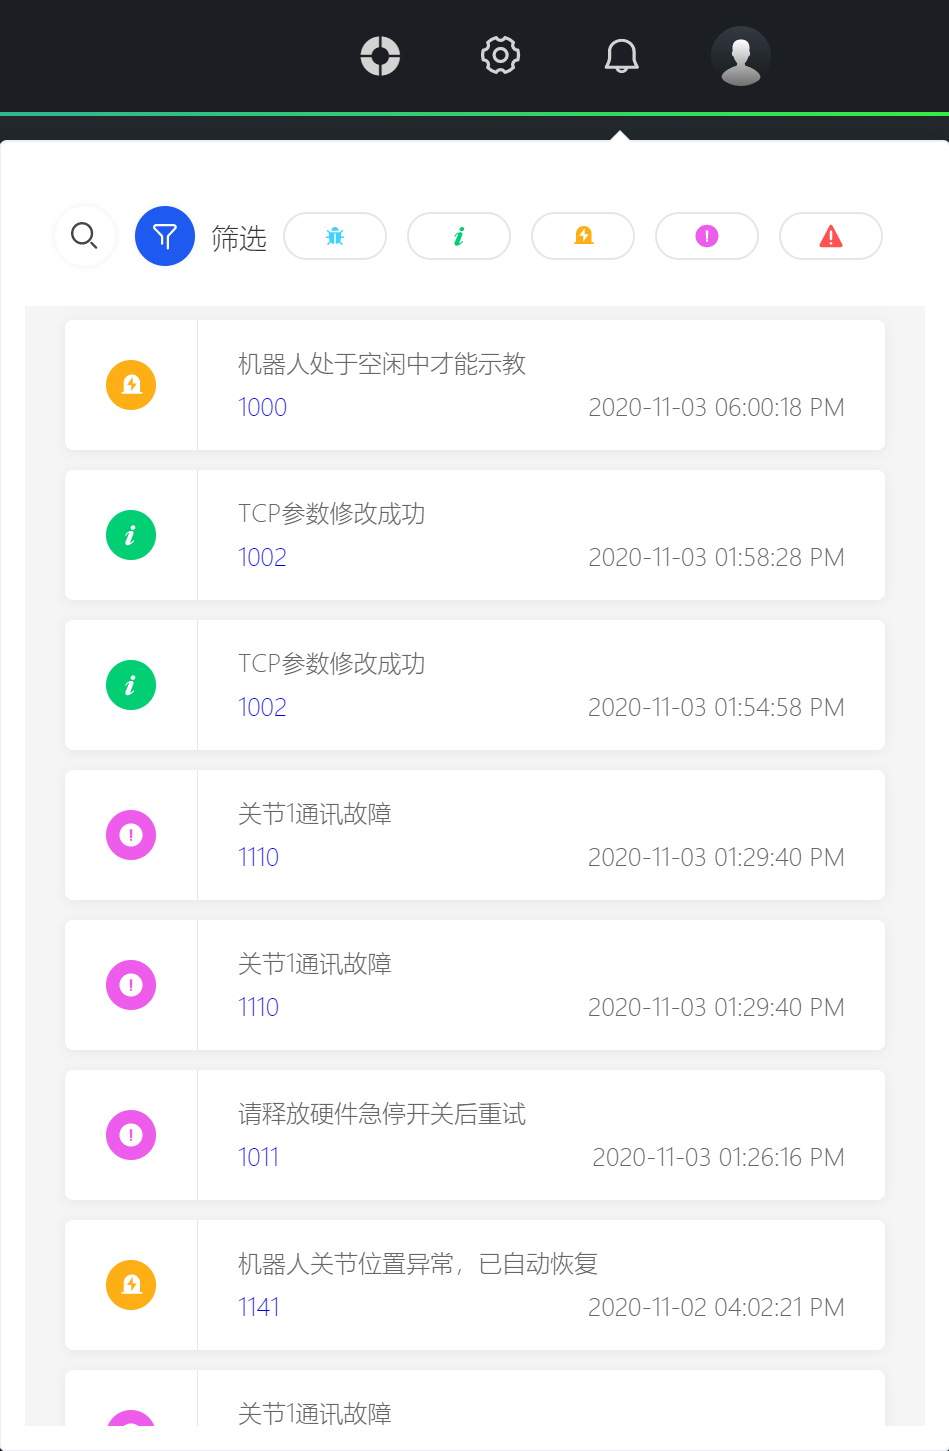
\includegraphics[height=8cm]{screen/2-14.png}
		\caption{消息中心}
		\label{fig:消息中心}
	\end{minipage}
	\hfill
	\begin{minipage}[t]{0.4\linewidth}
		\centering
		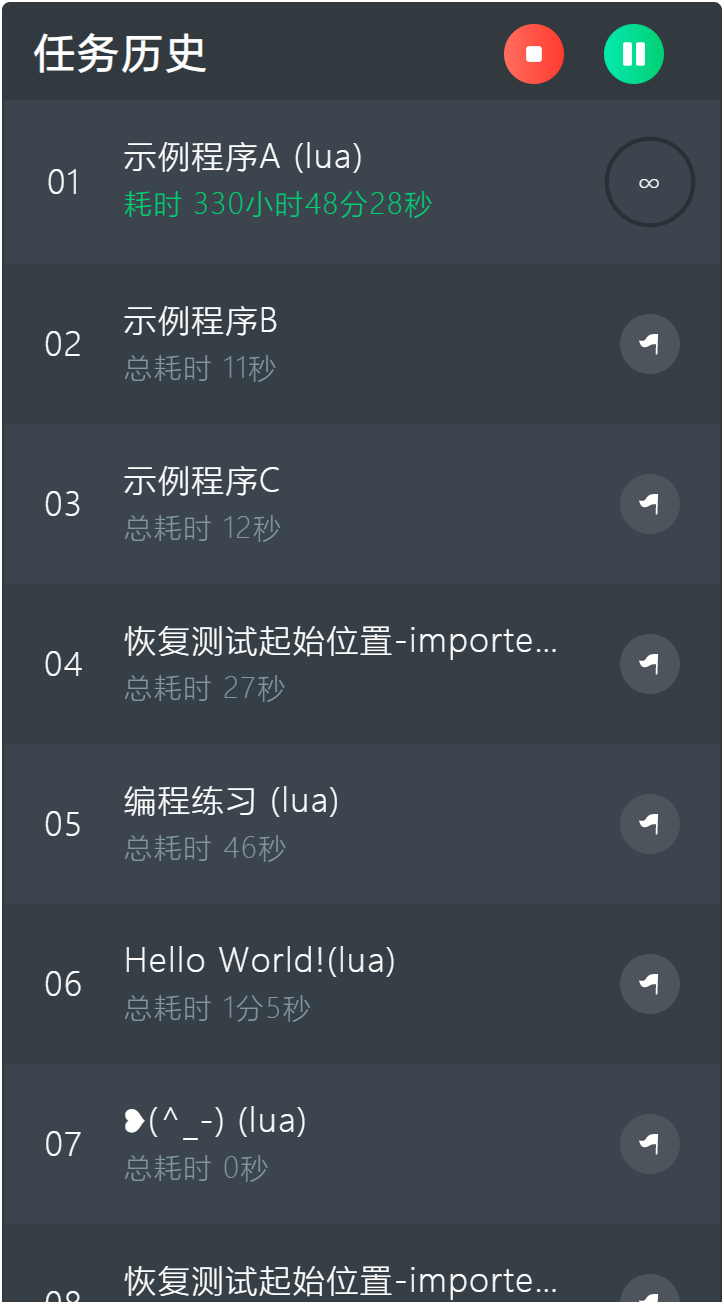
\includegraphics[height=8cm]{screen/2-15.png}
		\caption{任务历史}
		\label{fig:任务历史}
	\end{minipage}
\end{figure}

\clearpage

\section{启动机器人}
进入\LM ,如\prettyref{fig:启动机器人}所示,点击首页蓝色启动按钮\icn{image/39.pdf};当首页视图区上方机器人状态标签显示为\mnu{空闲}时,表示您已成功启动机器人。

\begin{figure}[ht]
	\centering
	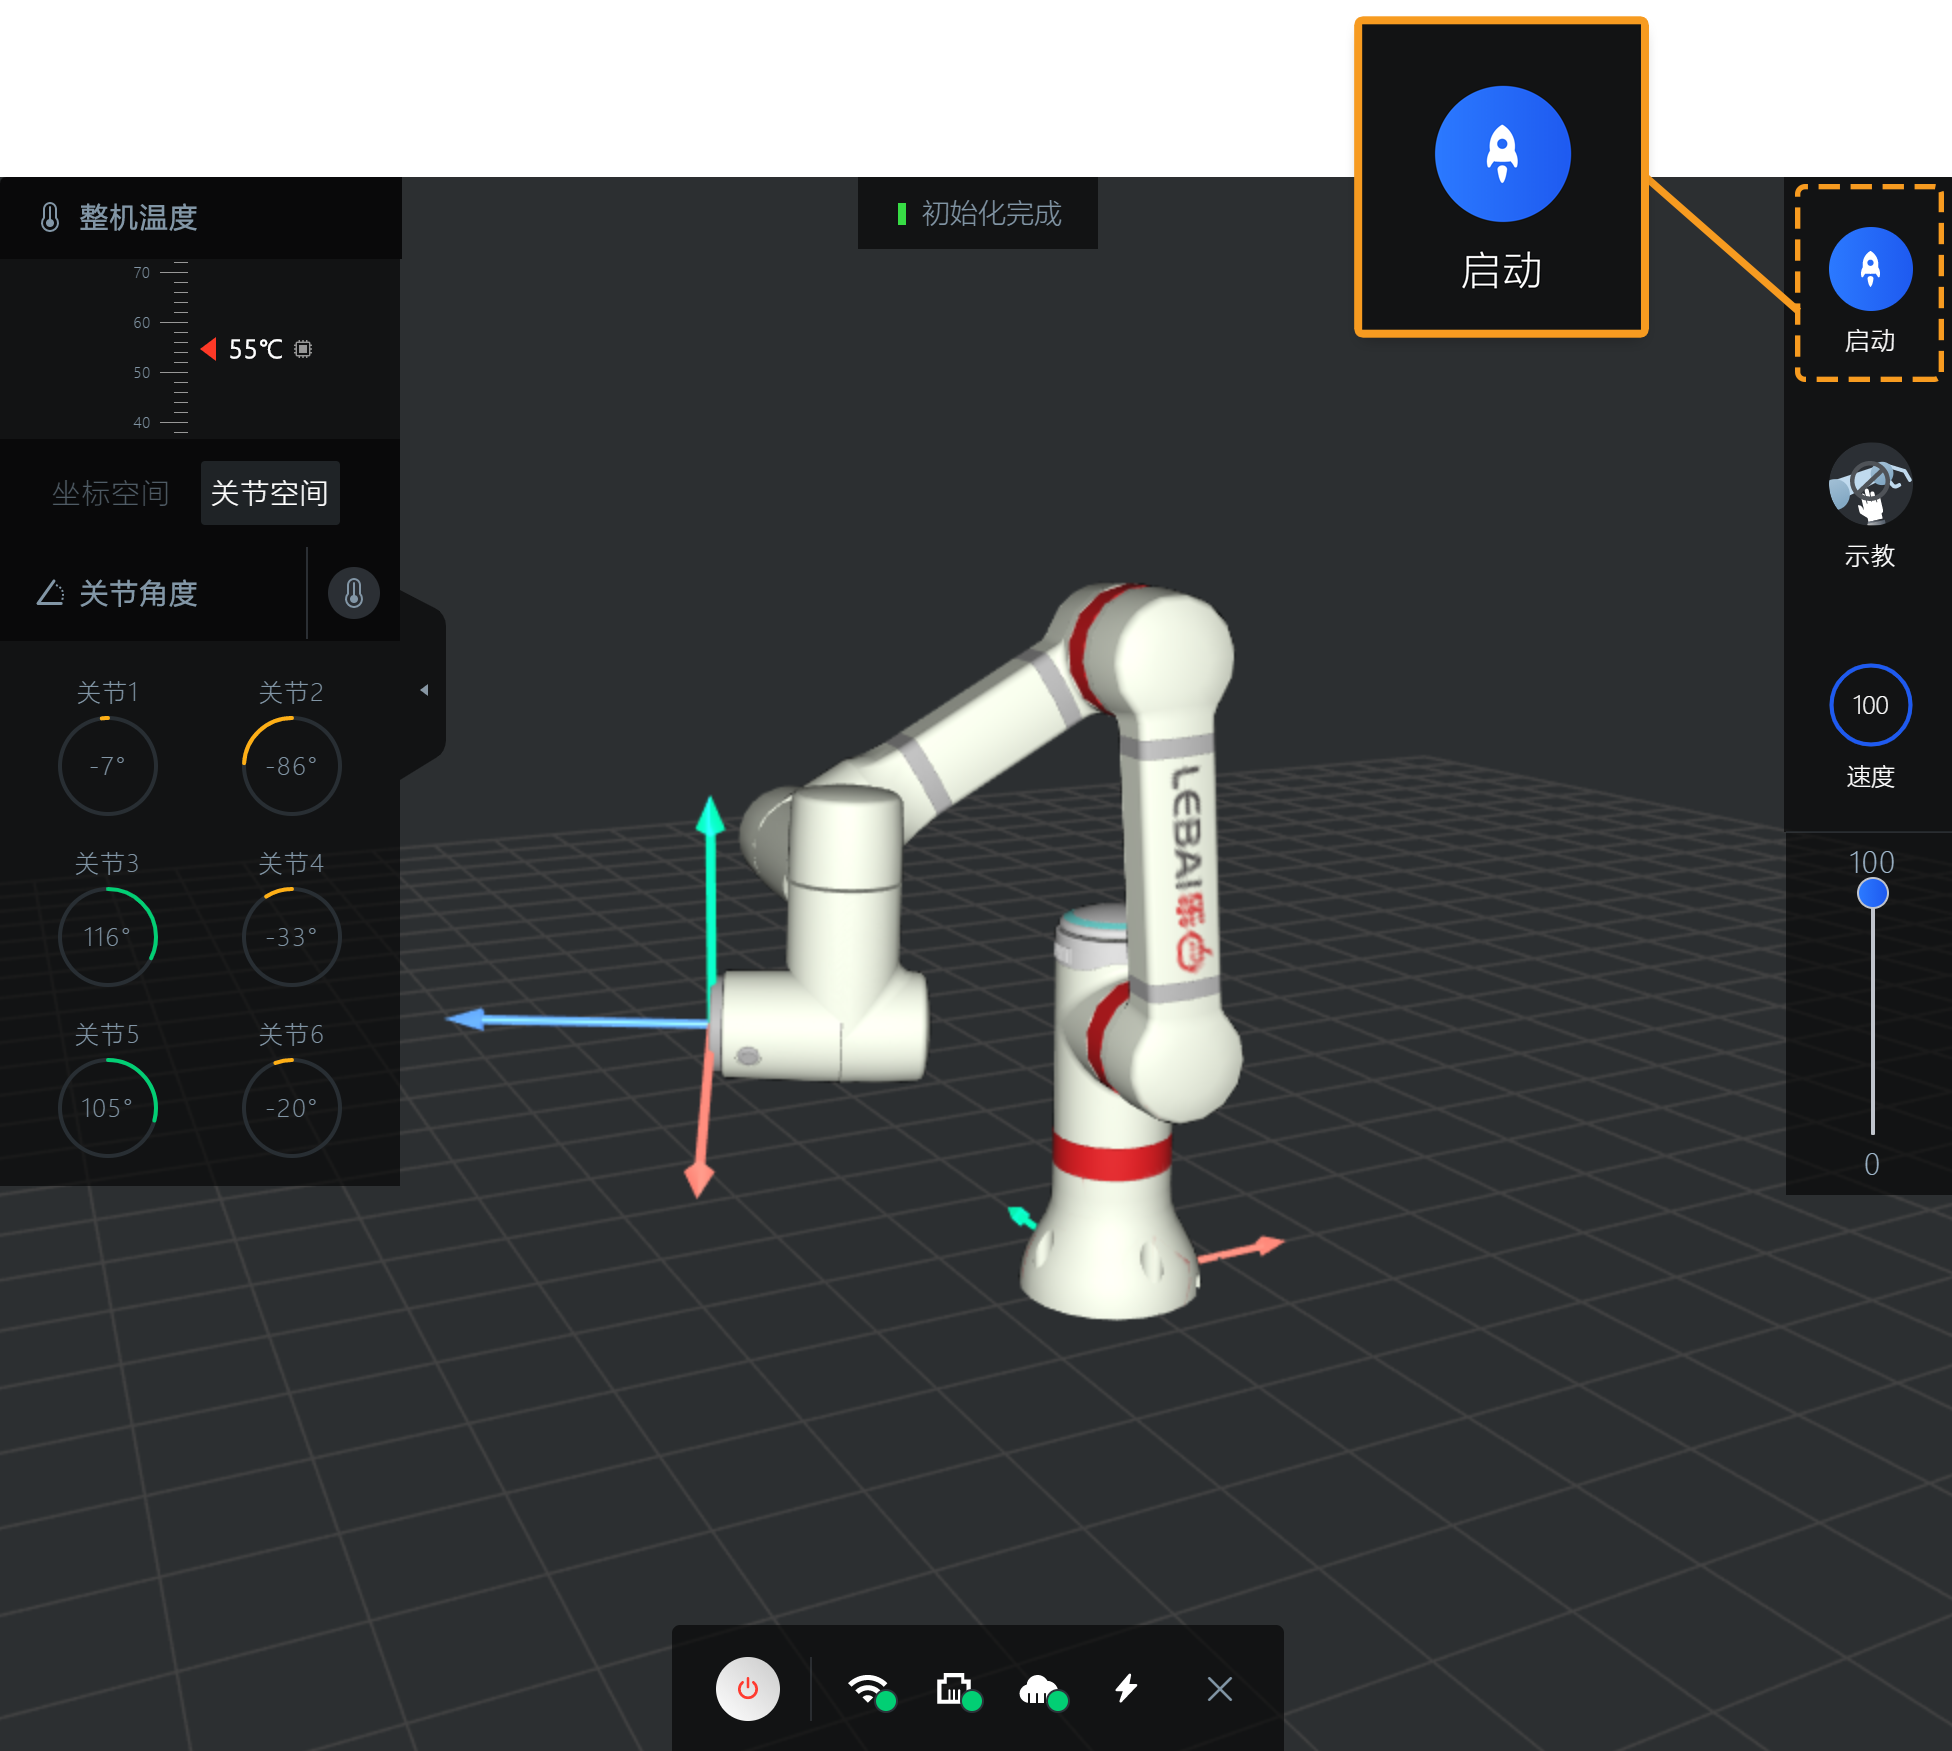
\includegraphics[width=\textwidth]{screen/2-16.png}
	\caption{启动机器人}
	\label{fig:启动机器人}
\end{figure}

\section{停止机器人}
当机器人处于\mnu{运行中}或\mnu{空闲}状态时,可以点击首页或如\prettyref{fig:胶囊控制区}所示的胶囊控制区的红色停止按钮;当机器人状态变为\mnu{已停止}时,表示您已成功停止机器人。

% \begin{figure}[ht]
% 	\centering
% 	\includegraphics[width=\textwidth]{image/6.pdf}
% 	\caption{\LM  首页--停止机器人}
% 	\label{fig:停止机器人}
% \end{figure}

\section{急停机器人}

急停操作有两种方式,可任选其一:
\begin{description}
	\item[软急停] \LM 右下方的红色\btn[Danger]{急停ESTOP}按钮;
	\item[硬急停] 按下控制箱顶部的红色凸起急停按钮或外接急停按钮(选配)。
\end{description}

\info{使用硬急停操作后,急停操作不会自动释放,需要顺时针旋转急停按钮,解除锁定后完成释放。}

\section{关闭机器人}
\begin{enumerate}
	\item 先停止或者急停机器人;
	\item 长按控制箱开关机按钮,直至蓝色灯光熄灭;
	\item 关闭控制箱背板的红色总电源开关。
\end{enumerate}

\danger[警告]{关闭机器人需严格遵守上述操作步骤,否则可能导致机器人文件系统损坏、机器人功能故障等问题。}

\section{胶囊控制区}
胶囊控制区仅在非首页时显示,可查看“机器状态”和“任务历史”。长按可拖动调整胶囊控制区在页面中的位置。

\begin{figure}[hb]
	\centering
	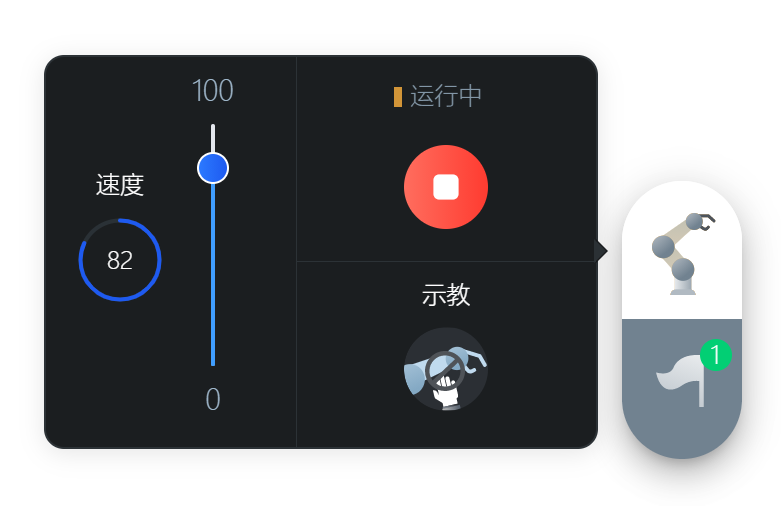
\includegraphics[height=4cm]{screen/2-18.png}
	\caption{胶囊控制区}
	\label{fig:胶囊控制区}
\end{figure}

\begin{description}
	\item [机器状态] 包含机器人当前状态、机器人启动/停止按钮、示教按钮以及速度调整拉杆,可以在非首页时操作和控制机器人;
	\item [任务历史] 包含正在运行中及已完成的任务列表、任务的暂停/恢复和停止按钮,可以在非首页时查看任务历史,具体操作见\prettyref{sec:任务历史}。
\end{description}
 % 3	基础操作
\appendix
\chapter{参照标准}
\label{app:参照标准}

乐白机器人LM3产品通过以下标准:

{\centering
\newcommand{\fenlei}[1]{\multirow{2}{5em}{\minitab[c]{#1}}}
\begin{tabularx}{\textwidth}{|m{5em}<{\centering}|l|>{\small}X|}\hline
\bf 分类    & \bf  标准    & \bf 定义\\\hline
\fenlei{电磁兼容\\标准}   &   GB/T17799.1-1999    &  电磁兼容通用标准居住、商业环境中的抗扰度试验\\\cline{2-3}
    &   GB/T17799.4-2001    &  电磁兼容通用标准工业环境中的发射\\\hline
    \fenlei{性能标准}    &   GB/T12642-2013  &  工业机器人性能规范极其试验方法\\\cline{2-3}
    &   GB/T20868-2007  &  工业机器人性能试验实施规范\\\hline
    安全标准    &   GB/T20867-2007  &  工业机器人安全实施规范\\\hline
    \fenlei{验收标准}    &   JB/T8896-1999   &  工业机器人验收规则\\\cline{2-3}
    &   JB/T10825-2008  &	工业机器人产品验收实施规范\\\hline
\end{tabularx}
}

 
\chapter{线上服务手册}

线上服务手册有以下两种获取方式,可任选其一:

\begin{itemize}
    \item 浏览器登录本公司官方网站:\url{https://lebai.ltd},进入“产品中心”,点击“文档库“,查看线上服务手册,了解更多;
    \item 扫描二维码,查看线上服务手册,了解更多。

    {\centering

    
\includegraphics[width=2.8cm]{image/qrcode.png} }
\end{itemize}
 % 附录 A 参照标准
\listoftables % 表格列表
\listoffigures % 图片列表
\printindex % 索引 makeindex
%\bibliography{...} % 参考文献 bibtex
\newcounter{int}
\setcounter{int}{2}
\begin{itemize}
\loop
\item[{\theint}.pdf] \includegraphics[height=2cm]{image/{\theint}.pdf}
\addtocounter{int}{1}
\ifnum \value{int}<45
\repeat
\end{itemize}

\end{document}
